\documentclass[12pt]{article}
\usepackage{sbc-template}
\usepackage{graphicx,url}
\usepackage[utf8]{inputenc}
\usepackage[brazil]{babel}
\usepackage{amsmath, amsfonts}
\usepackage{mathtools}  
\usepackage{float}
\usepackage{graphicx,url}
\usepackage{blindtext} 
\usepackage{lastpage}   
\usepackage{fancyhdr} 
\usepackage{graphicx}   
\usepackage{subcaption}  
\usepackage{multirow} 
\usepackage{tikz}  
\usepackage{listings}
\usepackage{xcolor} 
\usepackage{subcaption}

\definecolor{codegreen}{rgb}{0,0.6,0}
\definecolor{codegray}{rgb}{0.5,0.5,0.5}
\definecolor{codepurple}{rgb}{0.58,0,0.82}
\definecolor{backcolour}{rgb}{0.95,0.95,0.92}

\urlstyle{same} 
\pagestyle{fancy}
\fancyhf{}
\fancyhead[LE,RO]{}
\fancyhead[RE,RO]{\small{\thepage}}
\fancyfoot[CE,CO]{}
\fancyfoot[LE,RO]{}  

\usepackage{listings}
\renewcommand{\lstlistingname}{C\'{o}digo}
\usepackage{listingsutf8} 

\lstdefinestyle{mystyle}{
	backgroundcolor=\color{backcolour},   
	commentstyle=\color{codegreen},
	keywordstyle=\color{magenta},
	numberstyle=\tiny\color{codegray},
	stringstyle=\color{codepurple},
	basicstyle=\ttfamily\footnotesize,
	breakatwhitespace=false,         
	breaklines=true,                 
	captionpos=b,                    
	keepspaces=true,                 
	numbers=left,                    
	numbersep=5pt,                  
	showspaces=false,                
	showstringspaces=false,
	showtabs=false,                  
	tabsize=2
}

\lstset{style=mystyle}
\lstset{inputencoding=utf8} 
\lstset{literate=%
	{"}{{\textquotedbl}}1
	{é}{{\'{e}}}1
	{è}{{\`{e}}}1
	{ê}{{\^{e}}}1
	{ë}{{\¨{e}}}1
	{É}{{\'{E}}}1
	{Ê}{{\^{E}}}1
	{û}{{\^{u}}}1
	{ù}{{\`{u}}}1 
	{ú}{{\'{u}}}1
	{â}{{\^{a}}}1
	{à}{{\`{a}}}1
	{á}{{\'{a}}}1
	{ã}{{\~{a}}}1
	{Á}{{\'{A}}}1
	{Â}{{\^{A}}}1
	{Ã}{{\~{A}}}1
	{ç}{{\c{c}}}1
	{Ç}{{\c{C}}}1
	{õ}{{\~{o}}}1
	{ó}{{\'{o}}}1
	{ô}{{\^{o}}}1
	{Õ}{{\~{O}}}1
	{Ó}{{\'{O}}}1
	{Ô}{{\^{O}}}1
	{î}{{\^{i}}}1
	{Î}{{\^{I}}}1
	{í}{{\'{i}}}1
	{Í}{{\~{Í}}}1
} 



     
\sloppy

\title{Compilador da Linguagem T++}

\author{Rafael Rampim Soratto \inst{1}}


\address{Universidade Técnológica Federal do Paraná - UTFPR CM
  \email{soratto@alunos.utfpr.edu.br}
}

\begin{document} 

\maketitle

\begin{abstract}
The present work has the objective of structuring a compiler for the T ++ language. For this a process sequence is adopted: The first process is called lexical analysis, the expected result of this process is a list of tokens with the exact value of the meaning of a certain expression. After this process is performed the parsing of the language where the result is a syntactic tree.
\end{abstract}
     
\begin{resumo} 
  O presente trabalho possui o objetivo de estruturar um compilador para a linguagem T++. Para isso é adotada uma sequência de processos: O primeiro processo é chamado de análise léxica, o resultado esperado deste processo é uma lista de tokens com o valor exato do significado de certa expressão. Após este processo é realizada a análise sintática da linguagem onde o resultado trata-se de uma árvore sintática.
\end{resumo}
 

\section{Introdução} 
Um compilador é o responsável por receber um código fonte e transformar em um código alvo \cite{louden}. Para isso são realizados processos sequências que dividem as responsabilidades do compilador: 
\begin{enumerate}
	\item Análise Léxica; 
	\item Análise Sintática; 
	\item Análise Semântica; 
	\item Otimização de código fonte; 
	\item Gerador de código; 
	\item Otimizador de código alvo. 
\end{enumerate}  
A primeira parte do trabalho está relacionado com o processo de varredura realizado pela análise léxica, o resultado desse processo é uma lista de tokens gerados à partir de um código fonte fornecido. 
\subsection{Especificação da Linguagem T++}  
A linguagem T++ é um exemplo de código fonte que será passado para o compilador. O primeiro processo realizado neste código fonte é a varredura realizada pelo analisador léxico.  

Esta linguagem possui palavras reservadas para o seu funcionamento, elas são próprias da linguagem e sua sintaxe deve ser respeitada. Assim como as palavras reservadas existem símbolos que podem ser utilizados. Tanto as palavras reservadas e os símbolos precisam ser tratados pelo analisador léxico de maneira reconhecer todas as expressões da linguagem. Isto pode ser feito utilizando expressões regulares(autômatos finitos) \cite{automatos}. 


Os `tokens' e palavras reservadas utilizadas na linguagem são: 
\begin{figure}[H]   
	\centering
	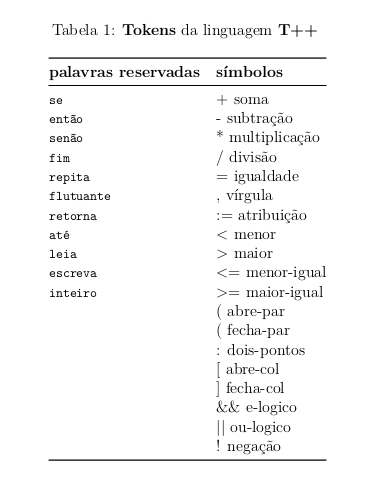
\includegraphics[scale=0.6]{tokens} 
	\label{tab:t1}
\end{figure} 

A linguagem não possui strings e todas as marcas ou são palavras reservadas ou símbolos. Tudo aquilo que não é palavra reservada mas começa com letra são identificadores (nome de funções, variáveis, etc). 

A linguagem T++ possui dois tipos de variáveis: inteiro e flutuante. Então os números podem assumir estes dois tipos. 
\section{Especificação formal dos Autômatos para as classes de token da linguagem} 
\label{sec:sx} 
Os autômatos representam as expressões regulares reconhecidas no processo de varredura. Ele é responsável por indicar quais expressões serão aceitas para que se gere o token respectivo da expressão. 

Construir o autômato de uma expressão regular permite visualizar com facilidade o funcionamento da expressão regular e também visualizar quais são os estados de aceitação do autômato. 

\subsection{Autômato para tratar dígitos} 
Quando se recebe um digito no arquivo .tpp ele pode ser enquadrar em qualquer uma das palavras reservadas e isso significa que o usuário está digitando um comando para ser interpretado.  

Caso esse digito não chegue no estado de aceitação de nenhuma palavra reservada então ele será tratado como `ID'. Este ID é útil para nomear variáveis, nome de funções e etc \ldots. 
O autômato que realiza o reconhecimento das palavras reservadas da linguagem em conjunto com reconhecimento dos ID's pode ser visualizado na figura \ref{fig:11}
\begin{figure}[H]  
	\centering
	\caption{Automato para reconhecer palavras reservadas e ID}
	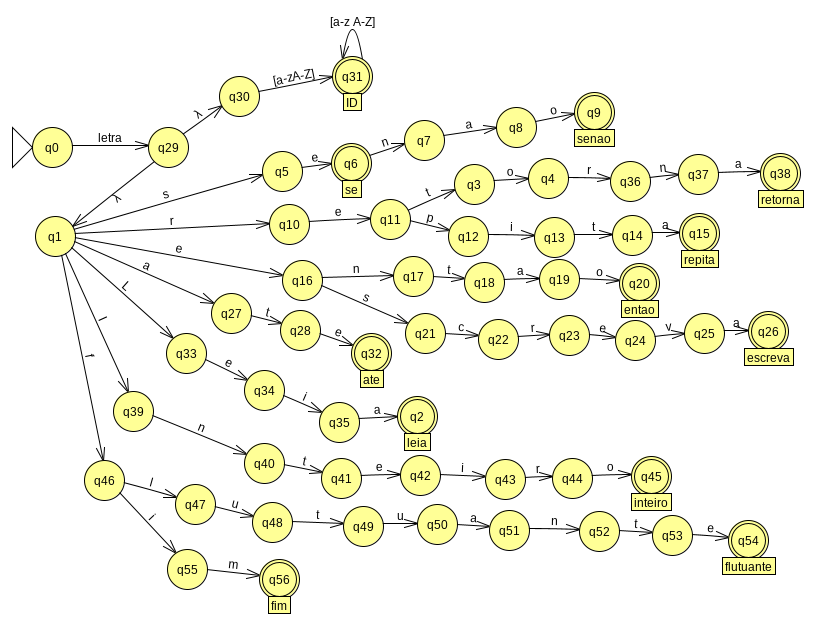
\includegraphics[scale=0.48]{automato.png} \\ 
	\textbf{Fonte :} Autoria Própria 2019.
	\label{fig:11}
\end{figure}   

De acordo com a figura\ref{fig:11} é possível visualizar que as palavras reservadas podem começar com os mesmos dígitos (e.g.repita e retorna), então seu reconhecimento começa igual e quando o digito é diferente criam-se sub-árvores para definir qual token será reconhecido. Isso também ocorre com as palavras `se' e `senão' que começam iguais porém uma sub-árvore é gerada para o senão por possuir dígitos diferentes.

\subsection{Autômato para tratar números}  
Quando recebe-se um número do teclado ou um símbolo de `+' ou '-' então isso significa que o token a ser gerado será um dos 3 tipos de números reconhecidos pela linguagem: inteiro, flutuante e notação científica. Lembrando que se a expressão começar com dígito então não há como ser classificado como número e o nome de uma variável também não pode começar com números.  
\begin{figure}[H]   
	\centering 
	\caption{Autômato para reconhecer inteiros, flutuantes e notações científicas}
	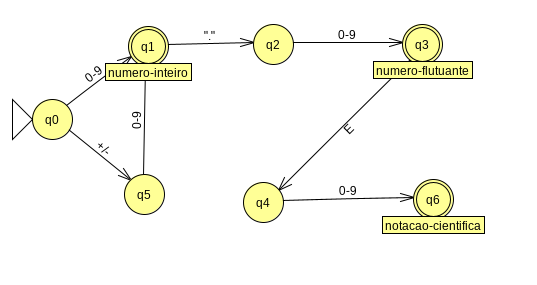
\includegraphics[scale=0.7]{numeros}\\ 
	\textbf{Fonte :} Autoria Própria (2019). 
\end{figure}  

\begin{figure}[H]  
	\centering 
	\caption{Autômato para reconhecer chaves,colchetes e comentários}
	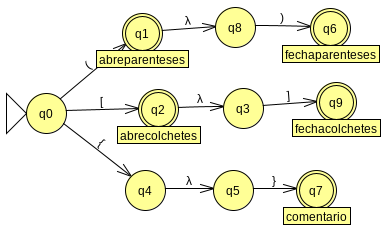
\includegraphics[scale=0.7]{chaves}\\ 
	\textbf{Fonte :} Autoria Própria (2019). 
	
\end{figure} 

\subsection{Autômato para tratar operadores lógicos, relacionais e de atribuição}  
Os símbolos reconhecidos pelo autômato e pelas expressões regulares tratam-se de operadores lógicos(e, ou, negação) e operadores relacionais (maior, maior igual, menor, menor igual). Também são tratados como símbolos os dois pontos e a atribuição (dois pontos seguido do sinal de igual). Todos operadores podem ser visualizados na Figura \ref{fig:ssim}:
\begin{figure}[H]  
	\caption{Autômato para reconhecer símbolos}
	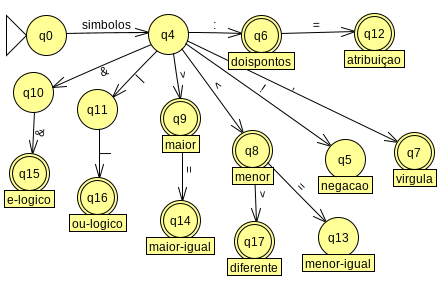
\includegraphics[scale=0.8]{simbolos}\\ 
	\textbf{Fonte :} Autoria Própria (2019). 	 
	\label{fig:ssim}
\end{figure}  

\subsection{Autômato para tratar operadores aritiméticos}  
Os operadores aritiméticos representam operações entre os números ou variáveis (soma, subtração, multiplicação, divisão), como ilustrado na Figura \ref{fig:ff}:
\begin{figure}[H]   
	\centering
	\caption{Autômato para reconhecer operações matemáticas}
	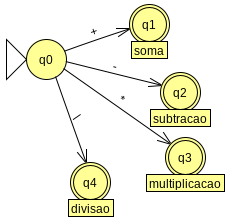
\includegraphics[scale=0.8]{operacoes}\\ 
	\textbf{Fonte :} Autoria Própria (2019). 	 
	\label{fig:ff}
\end{figure}    
\section{Implementação do Analisador Léxico}  
A função do analisador léxico é receber a linguagem T++ (código fonte) e de acordo com  o código lido deve ser gerada uma lista de \textit{tokens} correspondentes com cada expressão da linguagem.
O analisador léxico foi implementado utilizando a linguagem Python e o pacote PLY.  
\subsection{Lexer.py} 
Foi criado um pacote lexer.py para ser utilizado como ferramenta de análise léxica.
\begin{lstlisting}[language=Python, caption=Analisador Léxico]  
# -*- coding: UTF-8 -*-
import ply.lex as lex
from ply.lex import TOKEN
import sys
import re
# Palavras Rservadas
reserved = {
'se': 'SE',
'então': 'ENTAO',
'senão': 'SENAO',
'fim': 'FIM',
'leia': 'LEIA',
'escreva': 'ESCREVA',
'retorna': 'RETORNA',
'até': 'ATE',
'flutuante': 'FLUTUANTE',
'inteiro': 'INTEIRO',
'repita': 'REPITA',
}
# Lista de nomes dos tokens
tokens = [
# Logicals
'E', 'OU', 'NAO', 
# Types
'NUMERO_PONTO_FLUTUANTE', 'NUMERO_INTEIRO',
# Arithmeticals
'SOMA', 'SUBTRACAO', 'MULTIPLICACAO', 'DIVISAO',
# Relationals
'MENORIGUAL', 'MAIORIGUAL', 'IGUALDADE', 'DIFERENTE', 'MENOR', 'MAIOR',
# Simbolos
'VIRGULA', 'ATRIBUICAO', 'ABREPARENTESES', 'FECHAPARENTESES', 'ABRECOLCHETE', 'FECHACOLCHETE',
'ABRECHAVE', 'FECHACHAVE', 'DOISPONTOS',
# Outros
'ID', 'COMENTARIO']+list(reserved.values())

# NUMEROS
t_NUMERO_PONTO_FLUTUANTE = r'((\d+)(\.\d+)(e(\+|-)?(\d+))?|(\d+)e(\+|-)?(\d+))'
t_NUMERO_INTEIRO = r'\d+'
\end{lstlisting}

\subsubsection{Funções do Lexer} 
Além das palavras reservadas, símbolos e expressões regulares a classe Lexer possui duas funções essenciais: 
\begin{enumerate}
	\item Função para Buildar o Lexer; 
	\item Função para testar algum arquivo .tpp e retornar a lista de tokens.
\end{enumerate} 
Essas funções podem ser visualizadas no código a baixo: 
\begin{lstlisting}[language=Python, caption=Funções da Classe MyLexer em Python] 
lexer = lex.lex(debug=False) 

if __name__ == '__main__':
lista_tokens = []
new_token = {}
code = open(sys.argv[1])
code_text = code.read()
lex.input(code_text)
while True:
tok = lex.token()
if not tok:
break
new_token['Tipo'] = tok.type
new_token['Linha'] = tok.lineno
new_token['Valor'] = tok.value
lista_tokens.append(new_token)
print(new_token)
new_token = {}
\end{lstlisting} 

\section{Execução} 
Para executar um arquivo teste .tpp basta executar o arquivo principal `lexer' e passar o nome do arquivo. Isso gera uma lista de tokens relacionados com este arquivo passado. Pode-se ainda passar a opção `com' para gerar uma lista de tokens personalizada com o tipo e o nome dos tokens: 
\begin{itemize}
	\item python3 lexer.py teste.tpp 
\end{itemize}    

\subsection{Exemplo}  
\begin{lstlisting}[ caption=Insertion Sort em t++, label=cod:codinsertion]   
{recebe o vetor do usuario} 
inteiro: vet[100] 

recebeVetor(inteiro: n)
inteiro: i
i := 0
repita 
leia(vet[i])
i := i + 1
até i < n
fim

{ função insertion sort }
insertion_sort(inteiro: n) 
inteiro: i  
inteiro: j  
inteiro tmp  
i := 1
repita  
j := i 
repita  
tmp = vet[j] 
vet[j] = vet[j-1] 
vet[j-1] = tmp 
j := j - 1
até (j > 0) && (vet[j-1] > vet[j])
i := i +1  
até i < n 
fim

{funcao principal}
inteiro principal()
recebeVetor(10)
insertion_sort(10)
retorna(0)
fim
\end{lstlisting}
De acordo com o Código \ref{cod:codinsertion} podemos visualizar um arquivo.tpp contendo um algoritmo para ordenação de vetores ``\textbf{insertion sort}''.  

Para executar a tradução da linguagem e gerar a lista de tokens correspondentes (varredura) basta utilizar o comando : \\ 
\textbf{python3 lexer.py insertionsort.tpp}.   

Ao utilizar os comandos à cima será gerada lista de token. Na figura \ref{fig:fgh}: 
\begin{figure}[H]   
	\caption{Lista de tokens} 
	\centering
	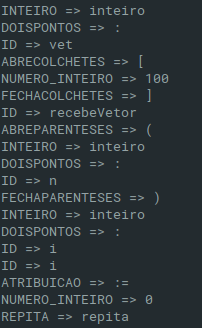
\includegraphics[scale=0.8]{resultado}\\ 
	\label{fig:fgh}
\end{figure}

\section{Analisador Sintático}  
A Análise Sintática determina a sintaxe ou estrutura de um
programa. A sintaxe de uma Linguagem de Programação é normalmente dada pelas regras gramaticais de uma gramática livre de contexto (GLC). Assim como a estrutura léxica é determinada por expressões regulares. 

Uma GLC utiliza convenções para nomes e operações muito similares
às usadas por expressões regulares, a diferença é que as regras de uma gramática livre de contexto podem ser recursivas (permite aninhamento de ifs). A classe de estruturas reconhecíveis por GLC é significativamente maior
que com Expressões Regulares. 

Existem duas categorias gerais de algoritmos para análise sintática: 
\begin{itemize}
	\item Análise Sintática Ascendente:  
	começa das folhas até a raiz (é a análise utilizada pelo pacote PLY do python também presente neste projeto); 
	\item Análise Sintática Descendente (deriva as regras da raiz para as folhas);
\end{itemize}
O Analisador Sintático ou `\textbf{parser}' é responsável por
determinar a estrutura sintática de um programa a partir das marcas (tokens) produzidos pelo processo de varredura (scanner) mostrado na seção anterior. O objetivo é
construir, explícita ou implicitamente, uma árvore sintática que representa essa estrutura. 

O analisador sintático pode ser visto como uma função de sequências
de marcas produzidas pela varredura para a árvore sintática. Nem todas as sequências de tokens são programas válidos, o analisador sintático tem que distinguir entre sequências válidas e
inválidas. 
  
\subsection{Gramáticas Livres de Contexo} 
Como apresentado na seção \ref{sec:sx} durante o processo de análise léxica são utilizadas expressões regulares. Porém, na análise sintática não podemos utilizar expressões regulares pois não há como definir a precedência de operadores. Para resolver este problema são utilizadas as gramáticas livres de contexto, notação `mais poderosa'. 

Uma Gramática Livre de Contexo (CFG) é composta por:  
\begin{itemize}
	\item Conjunto de terminais T; 
	\item Conjunto de não terminais V; 
	\item 1 não terminal inicial S; 
	\item Um conjunto de produções P;   
	\subitem
	- 	Uma produção é um par de um não-terminal e uma cadeia
	(possivelmente vazia) de terminais e não-terminais
	 
	\subitem -  
	Podemos considerar produções como regras; o não-terminal é o lado
	esquerdo da regra e a cadeia é o lado direito 
	\item Existe a linguagem denotada pela gramática G:L(G).
\end{itemize} 
\subsection{Formato da Análise sintática LALR(1)} 
De acordo com \cite{yacc} o Yacc (yet another compiler-compiler) é
um gerador automático de Analisadores Sintáticos do tipo LALR(1). A maioria das ferramentas de análise sintática são
expressadas convenientemente por analisadores LALR(1) pois ela permite diminuir os estados da tabela de símbolos do LR(1). Logo é construída uma máquina de estados referente a linguagem e então passa as informações de estados e transições para uma tabela de símbolos. Nesta tabela encontram-se os estados e para cada símbolo a célula da tabela mostra pra qual estado ir \dots A diferença é que os estados iguais são unidos em um único estado na utilização do LALR. 
\subsection{Implementação e Yacc} 
O Yacc trabalha em conjunto com o Lex, o que é possível de ser visualizado na Figura: 
\begin{figure}[H]  
	\centering 
	\caption{Funcionamento do Yacc} 
	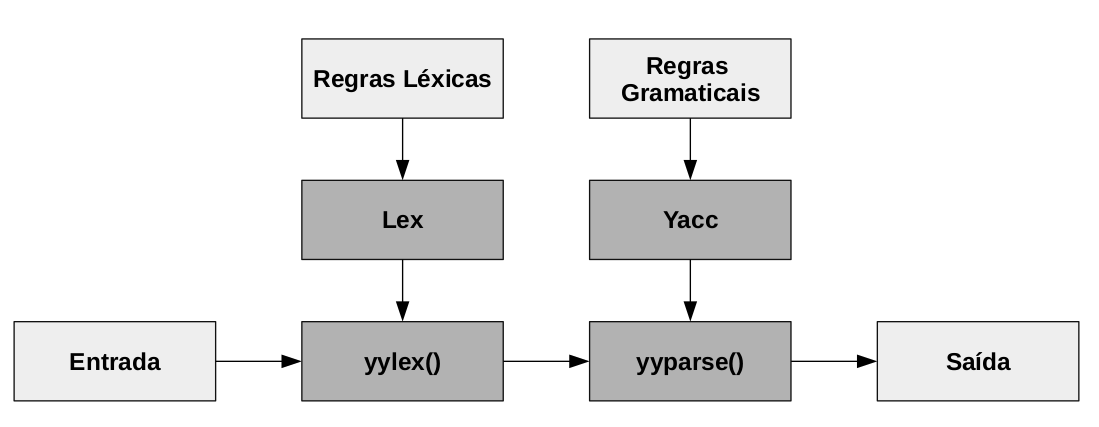
\includegraphics[scale=0.4]{func}
\end{figure}  
  
\subsection{Implementação da Árvore Sintática} 
Uma Árvore de Análise Sintática ou Árvore de `parse' é uma árvore
rotulada que possui:  
\begin{itemize}
	\item não-terminais nos nós interiores
	\item nós-folha são terminais
	\item filhos de cada nó interno representam a substituição do não-terminal associado ao passo de derivação.
\end{itemize}
Percorrer a árvore em ordem dá a cadeia sendo derivada
A árvore sintática dá a estrutura e associatividade das operações que a cadeia original não mostra. 
Para construir a arvore em Python foi utilizada a estrutura de nós fornecida  pelo pacote \textbf{anytree}. A raiz da árvore representa o programa principal e as folhas representam as variáveis e ID's.   
 
Para cada token lido será gerada uma sub-árvore que representa uma regra. No final, quando todos tokens passarem pelo processo de `\textbf{parse}' então é esperável que todas as sub-árvores possuam como raiz o programa pŕincipal, `\textit{main}'. Desta forma, basta imprimir a raiz que representa o programa para visualizar a árvore sintática do programa.  

\begin{lstlisting}[language= Python, caption=Criação de Nós na Árvore Sintática, label=cod:codd] 
def criar_variavel(pai,line2,p): 
	return Node('ID-' + p[1], parent=pai, line=line2)       

# arvore sintática é implementada com nós 
# um nó tem as seguintes informacoes:  
# (nome, pai, numero)
def criar_no(name, parent=None, line=None):
# estrutura para mostrar o número e o tipo do nó
	if parent and line:
		return Node(name, parent=parent, line=line) # ID
	elif parent:
		return Node(name, parent=parent)
	else:
		return Node(name)    
\end{lstlisting}
 
\begin{lstlisting}[language= Python, caption= Função de Erros e Main do Parser, label=cod:coddp] 
 
# funcao de erro
def p_erro(p): 
# se for error de sintaxe    
	if p: 
# mostra uma exeção indicando a linha e o token     
# # print('Erro sintático na linha %d - Posição %d: '%s'' % (p.lineno, p.lexpos, p.value))     
	raise Exception('Erro sintático na linha {} no token '{}''.format(p.lineno, p.value))
	else: 
	# reinicia o parser    
		parser.restart()  
		print('Erro sintático nas definições!')
		exit(1)
# gera uma  execao de erro
		raise Exception('Erro')  
		
if __name__ == '__main__': 
# main 
#  
# ativa o parser  
parser = yacc.yacc(debug=True, tabmodule='fooparsetab') 
#recebe o arquivo com códgio tpp
code = open(sys.argv[1]) 
# le arquivo
code_text = code.read() 
# realiza a analise sintatica do código
try:
result = parser.parse(code_text, debug=False)  
print('A raíz do programa: ',result) 
except Exception as e:
raise e 
code.close()
# se houver uma raiz então pode-se mostrar a ávore sintática dessa raiz 
# se não houver uma raíz possui erro de construção sintática  
if (raiz):   
print('Gerando imagem da árvore...')
DotExporter(raiz).to_picture('arvore-sintatica.png') 
else:
raise Exception('Houve erro ao tentar gerar a árvore' 
\end{lstlisting}
\subsection{Exemplo de saída (árvore sintática)}   
\begin{figure}[H]  
	\centering  
	\caption{Árvore Sintática}
	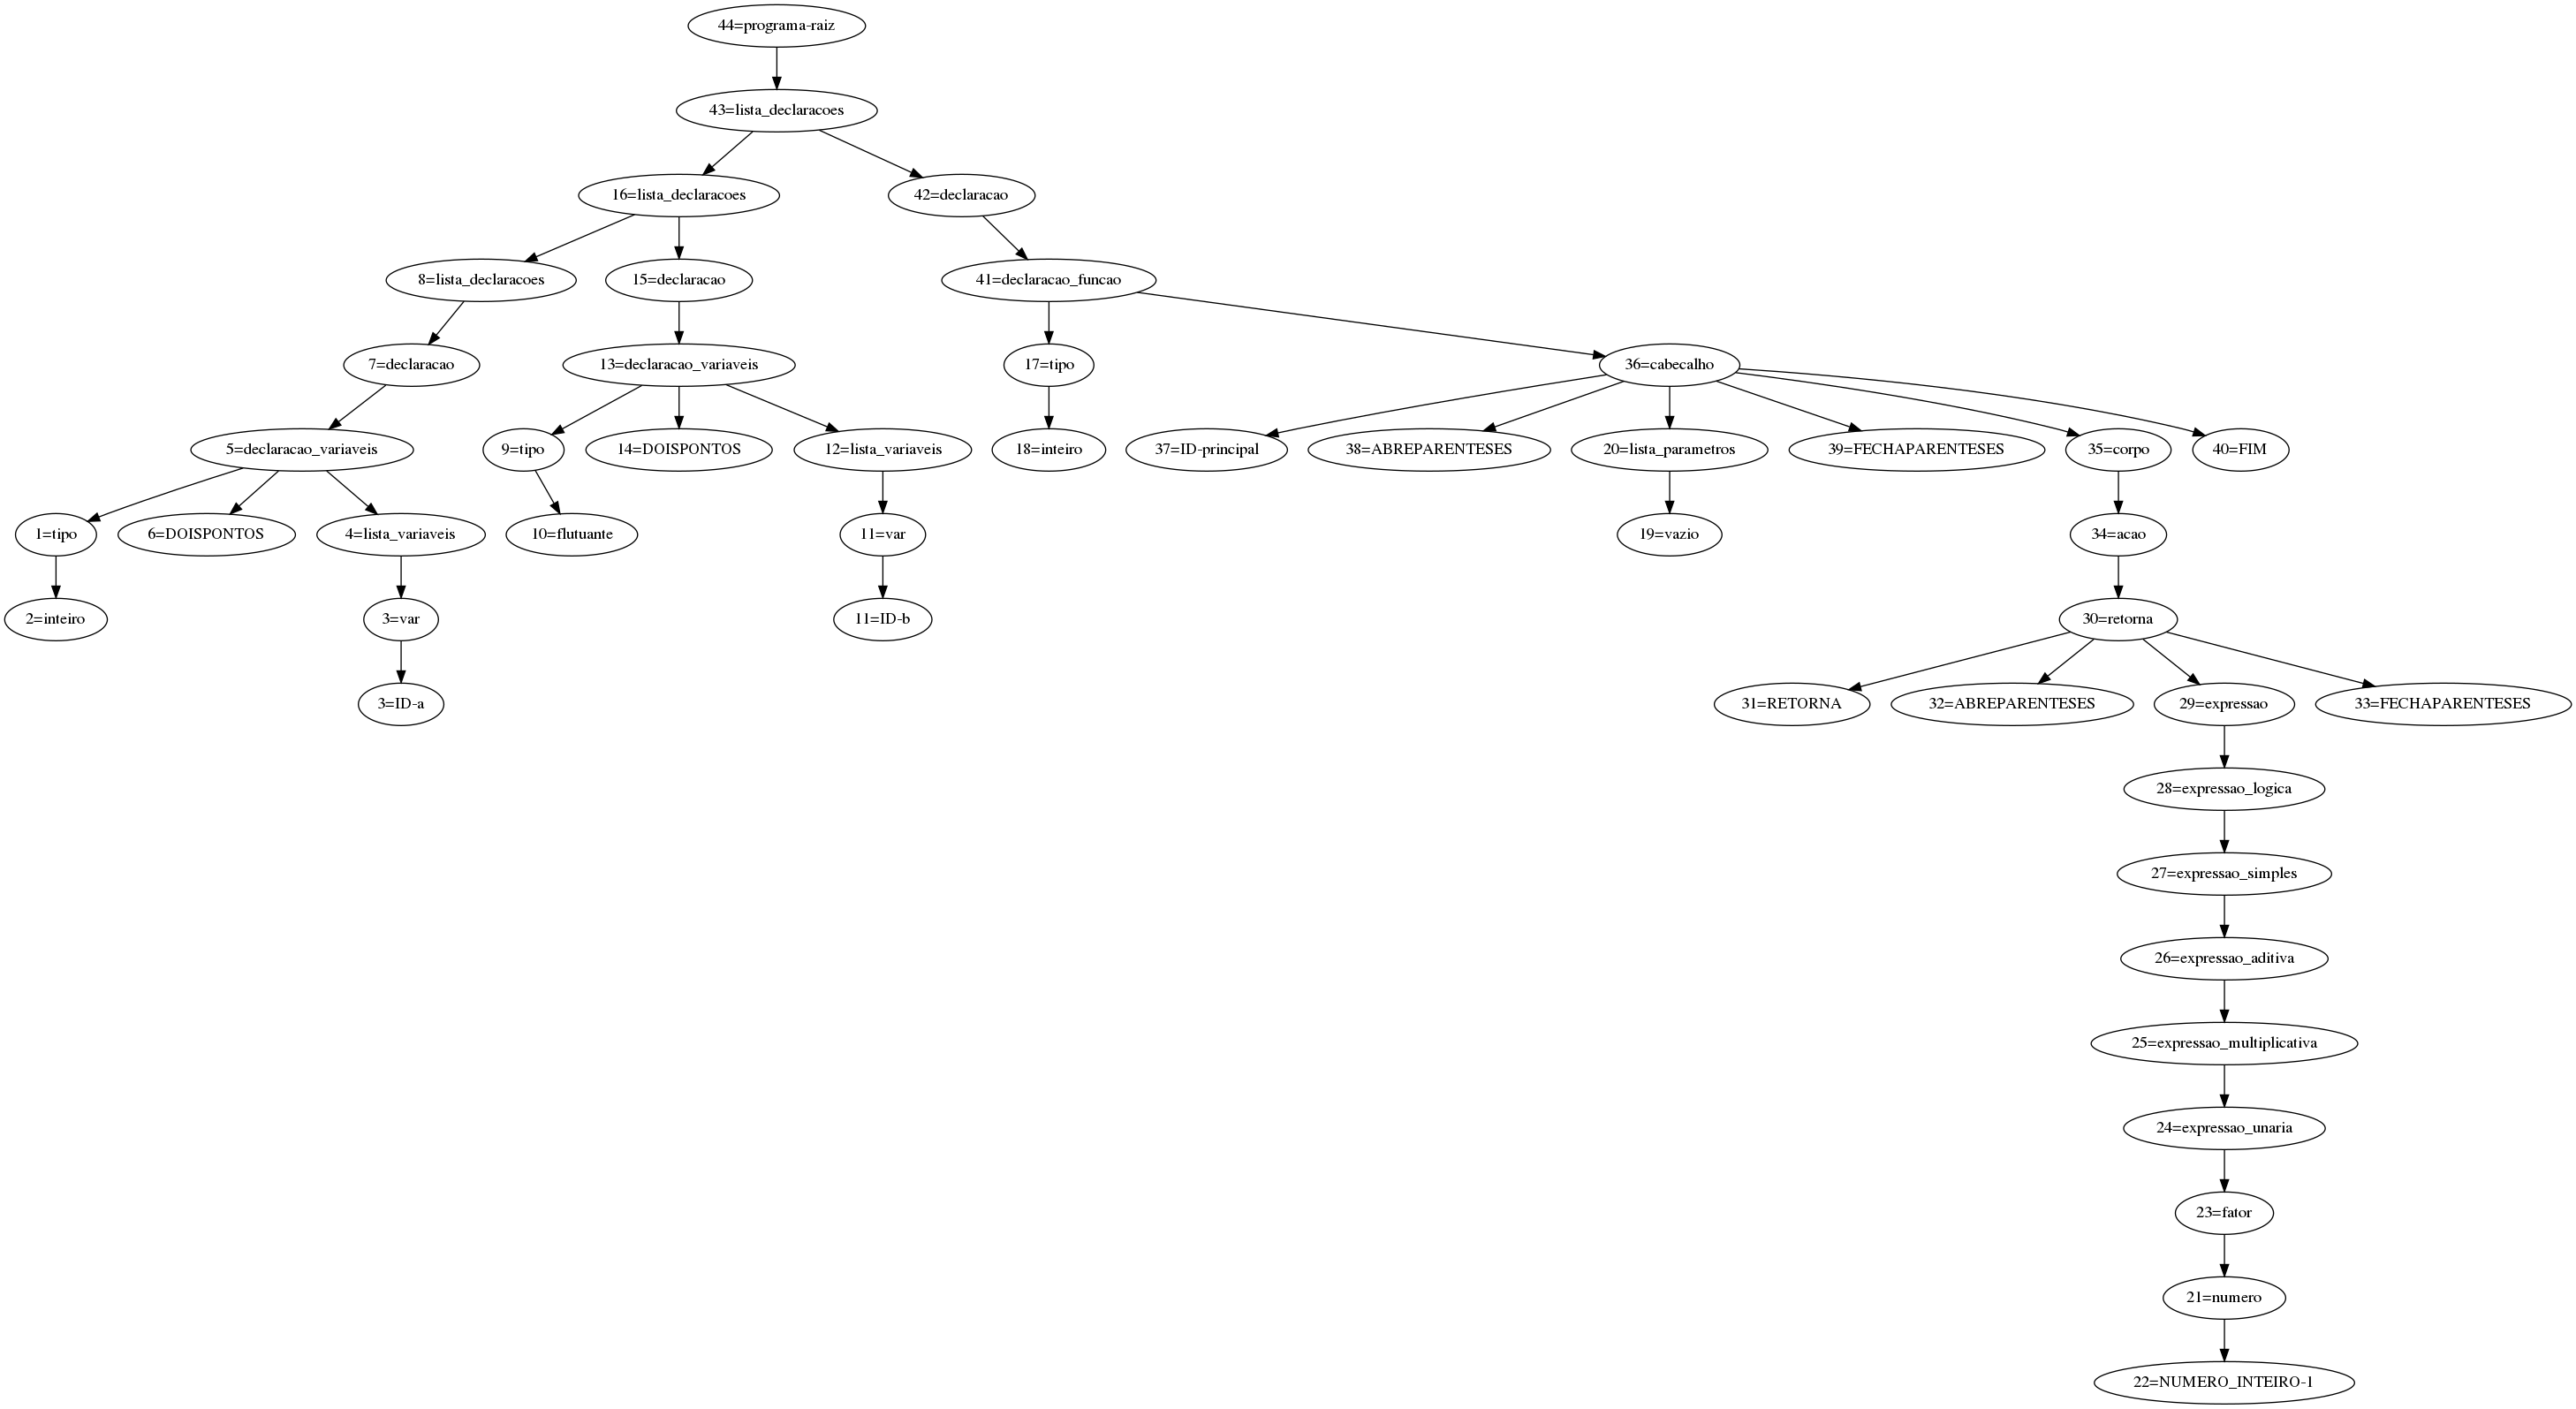
\includegraphics[width=\textwidth, height=\textheight]{arvore-sintatica1} 
	\label{fig:arvoresimplificada1}
\end{figure} 
    

\section{Análise Semântica}  
Dado que a árvore sintática foi construída sintaticamente de maneira correta, podemos construir uma tabela de símbolos contendo algumas informações essenciais sobre as variáveis e as funções do programa: 

\begin{itemize}
	\item \textbf{Funções, Procedimentos e Variáveis}:\\ O identificador de função (nome e quantidade de
	parâmetros formais), além de que os parâmetros formais devem ter um apontamento
	para o identificador de variáveis. 
	O identificador de variáveis locais e globais: nome, tipo e escopo
	devem ser armazenados na Tabela de Símbolos. Variáveis devem ser declaradas,
	inicializadas e antes de serem utilizadas (leitura). Lembrando que uma variável pode
	ser declarada no escopo global ou no escopo de uma função ou procedimento. Durante a criação da tabela de símbolos todas essas informações devem ser atribuídas nas variáveis e funções: 
	\begin{itemize}
		\item Token (id ou func); 
		\item Tipo; 
		\item Nome; 
		\item Linha; 
		\item Dimensão (arrays); 
		\item Retorno (funções); 
		\item Estado; 
		\item Número de parâmetros reais e formais (funções);
	\end{itemize}
Para armazenar, as funções e as variáveis é utilizada uma tabela de símbolos implementada como um dicionário em Python. 

\end{itemize} 

Com a tabela de símbolos construída e a árvore sintática correta é possível realizar as verificações semânticas do programa: 
\begin{enumerate}
\item \textbf{Função Principal}: todo programa precisa ter uma função principal que retorna um valor inteiro.  
	\item \textbf{Parâmetros de uma função}: A quantidade de parâmetros reais de uma chamada de
	função/procedimento func deve ser igual a quantidade de parâmetros formais da sua
	definição. 
	\item \textbf{Retorno da Função}: o tipo de retorno da função deve ser equivalente ao tipo de declaração da função.  
	\item Uma função qualquer não pode fazer uma chamada à função principal. Se a função principal fizer uma chamada para ela mesmo, a mensagem de aviso deve ser
	emitida. 
	\item Uma função pode ser declarada e não utilizada. Se isto acontecer uma aviso deverá ser
	emitido. 
	\item \textbf{Variáveis}: 
	A variável que foi declarada deve ser utilizada. Se a variável for utilizada sem ser declarada deve mostrar um erro. Não se pode declarar duas variáveis com o mesmo nome. 
	\item \textbf{Atribuições e Coerções implícitas}: As atribuições entre variáveis deve ser compatível, ou seja, uma variável inteiro deve receber um inteiro ou algo que retorne um inteiro. Da mesma forma para as variáveis do tipo flutuante. Porém não é gerado um erro quando isso ocorre, apenas um aviso... A diferença é que os avisos não interrompem a execução do programa como fazem os erros. 
	\item \textbf{Arranjos e Arrays}: Os vetores na linguagem tpp não podem ter o índice flutuante caso contrário deve-se retornar um erro. Se o array é definido com o índice 2 então na utilização desse vetor não se pode exceder o índice formal. Neste caso o erro (index out of range) é mostrado. 
	  
\end{enumerate} 

De acordo com a lista de erros e avisos que o analisador semântico deve mostrar para o usuário da linguagem Tpp é garantida que a árvore do programa não possua erros de funcionamento podendo então prosseguir para a fase de geração de código intermediário. 
Portanto a entrada do processo de análise semântica é a árvore gerada na sintática que é analisada na semântica utilizando uma tabela de símbolos como apoio e então gerando uma árvore coerente à um programa executável. 
O código que representa isso é: 
\begin{lstlisting}[language= Python, caption= Funções semânticas, label=cod:coddp] 
# se houver uma raiz então pode-se mostrar a ávore sintática dessa raiz 
# se não houver uma raíz possui erro de construção sintática  
if (raiz):    

	DotExporter(raiz).to_picture(arvore-sintatica1.png)   
	# lista as funcoes e variáveis do programa 
	tableofsymbols = tabela_variaveis(raiz)
	#print(tableofsymbols)  
	verify_main(tableofsymbols) 
	verify_functions(tableofsymbols,raiz) 
	verify_variables(tableofsymbols,raiz)   
	verify_index_var(tableofsymbols,raiz)
	verify_assignments(tableofsymbols,raiz) 
	simplify_tree(raiz) 
	 
	DotExporter(raiz).to_picture(arvore-sintatica2.png)    
else:
	raise Exception('Houve erro ao tentar gerar a árvore')  
\end{lstlisting} 

\section{Exemplo de utilização}  
Com o simples exemplo de código na linguagem tpp: 
\begin{lstlisting}[ caption= Código em TPP, label=cod:coddp] 
{Aviso: Variável 'a' declarada e não utilizada}
{Aviso: Variável 'b' declarada e não utilizada}
inteiro: a
flutuante: b
inteiro principal() 
	retorna(1) 
fim  
\end{lstlisting} 

Obtemos a tabela de símbolos e os avisos correspondentes: 
\begin{figure}[H] 
	\centering  
	\caption{Tabela de símbolos e funções}
	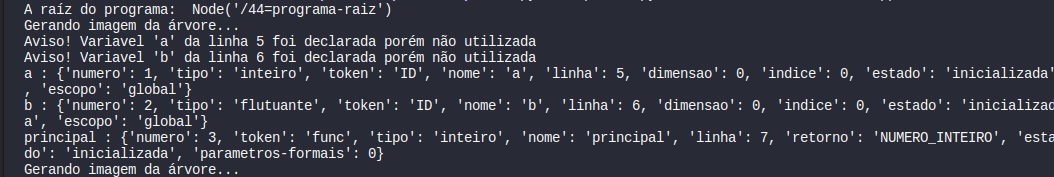
\includegraphics[scale=0.4]{tableofsymbol.png} 
	\label{fig:table}
\end{figure} 
De acordo com a figura  
\ref{fig:table} é possível visualizar que as variáveis são implementadas em tuplas na linguagem Python e cada tupla possui os atributos: 
\begin{itemize}
	\item Número 
	\item Tipo: tipo da variável é inteiro ou flutuante; 
	\item Token: ID se for variável e func se for função; 
	\item Nome: nome da variável ou da função; 
	\item Linha; 
	\item Dimensão: 0 se for variável e 1 se for vetor, assim consecutivamente\ldots 
	\item Índice: O tamanho do array. Se for variável é 0. 
	\item Estado: inicializada ou utilizada. 
	\item Escopo: nome da função onde foi declarada ou global.
\end{itemize} 
A diferença entre as tuplas de variáveis e funções é que as funções possuem os atributos: 
\begin{itemize}
	\item Retorno: tipo do retorno; 
	\item Número de parâmetros formais e reais;  
	\item Retorno real utilizado ao ser chamada. Utilizado para comparar o tipo de retorno real com o definido na declaração da função.
\end{itemize} 
Ainda na Figura \ref{fig:table} é possível visualizar dois avisos sobre o programa que refere-se a duas variáveis definidas e não utilizadas.  
Se não houver erros semânticos então o resultado será duas árvores: uma completa e uma simplificada: 
\begin{figure}[H]  
	\centering  
	\caption{Árvore completa}
	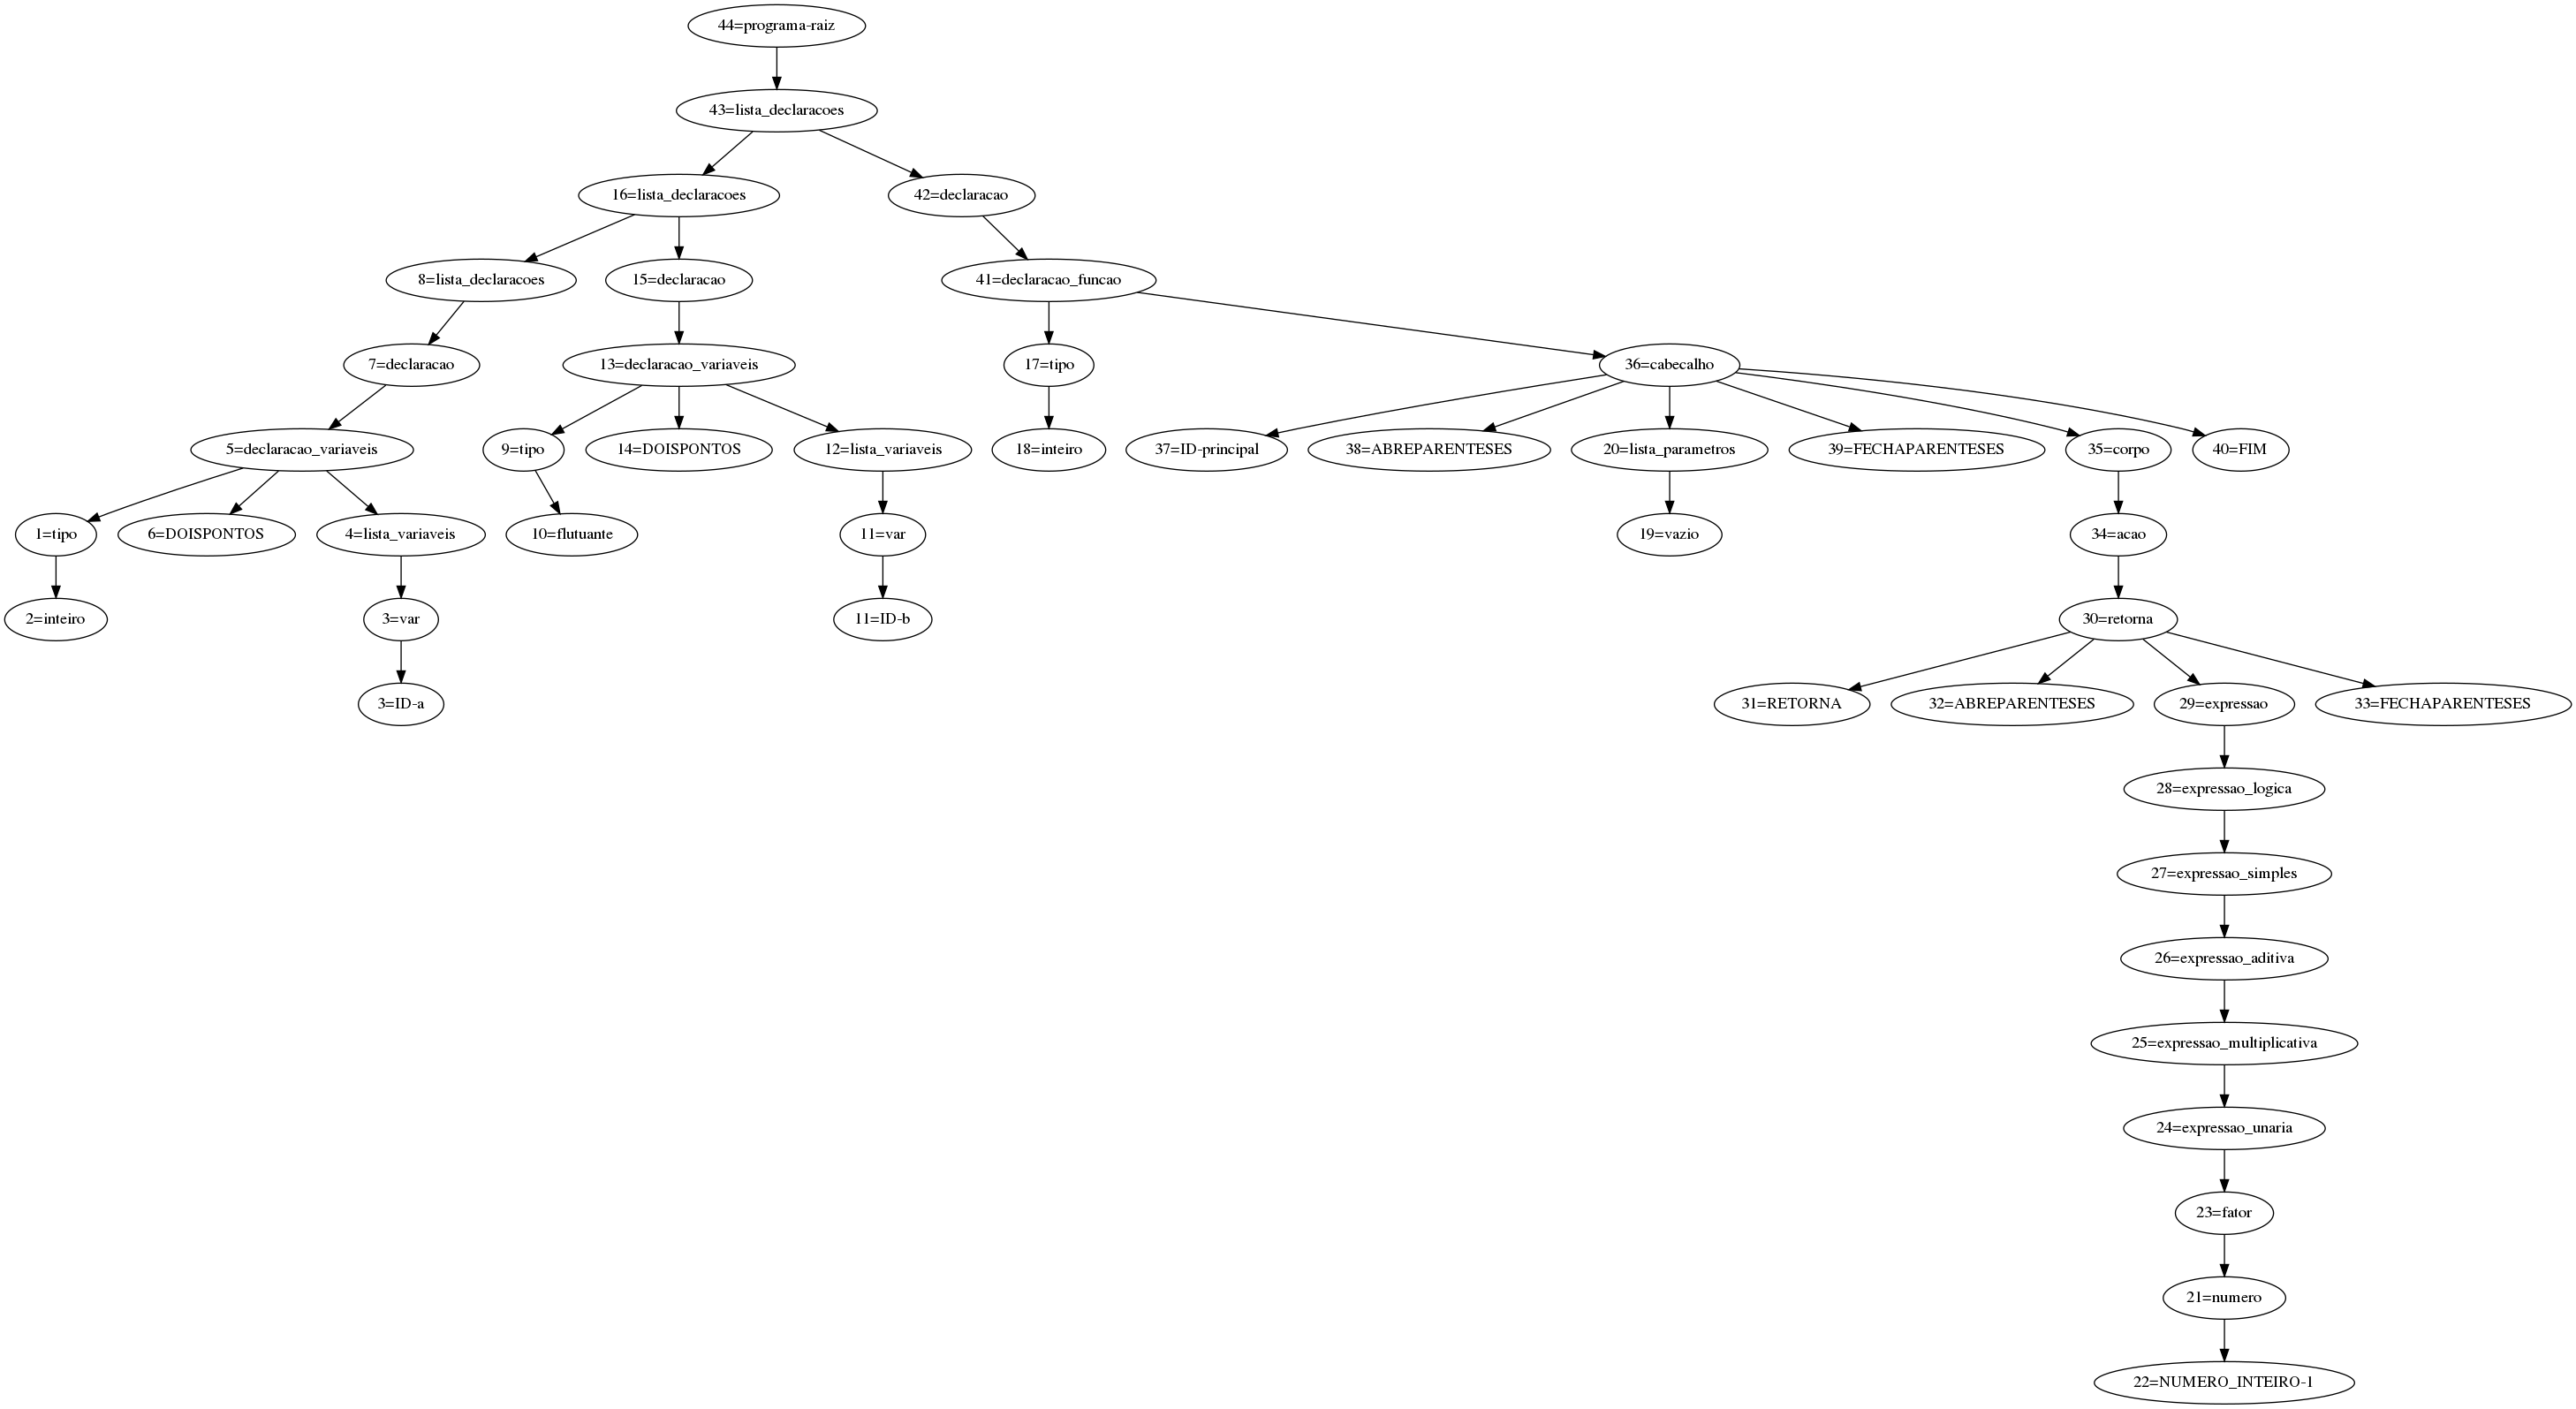
\includegraphics[width=\textwidth]{arvore-sintatica1} 
	\label{fig:arvorecompleta}
\end{figure}

\begin{figure}[H]  
	\centering  
	\caption{Árvore Simplificada sem erros Semânticos}
	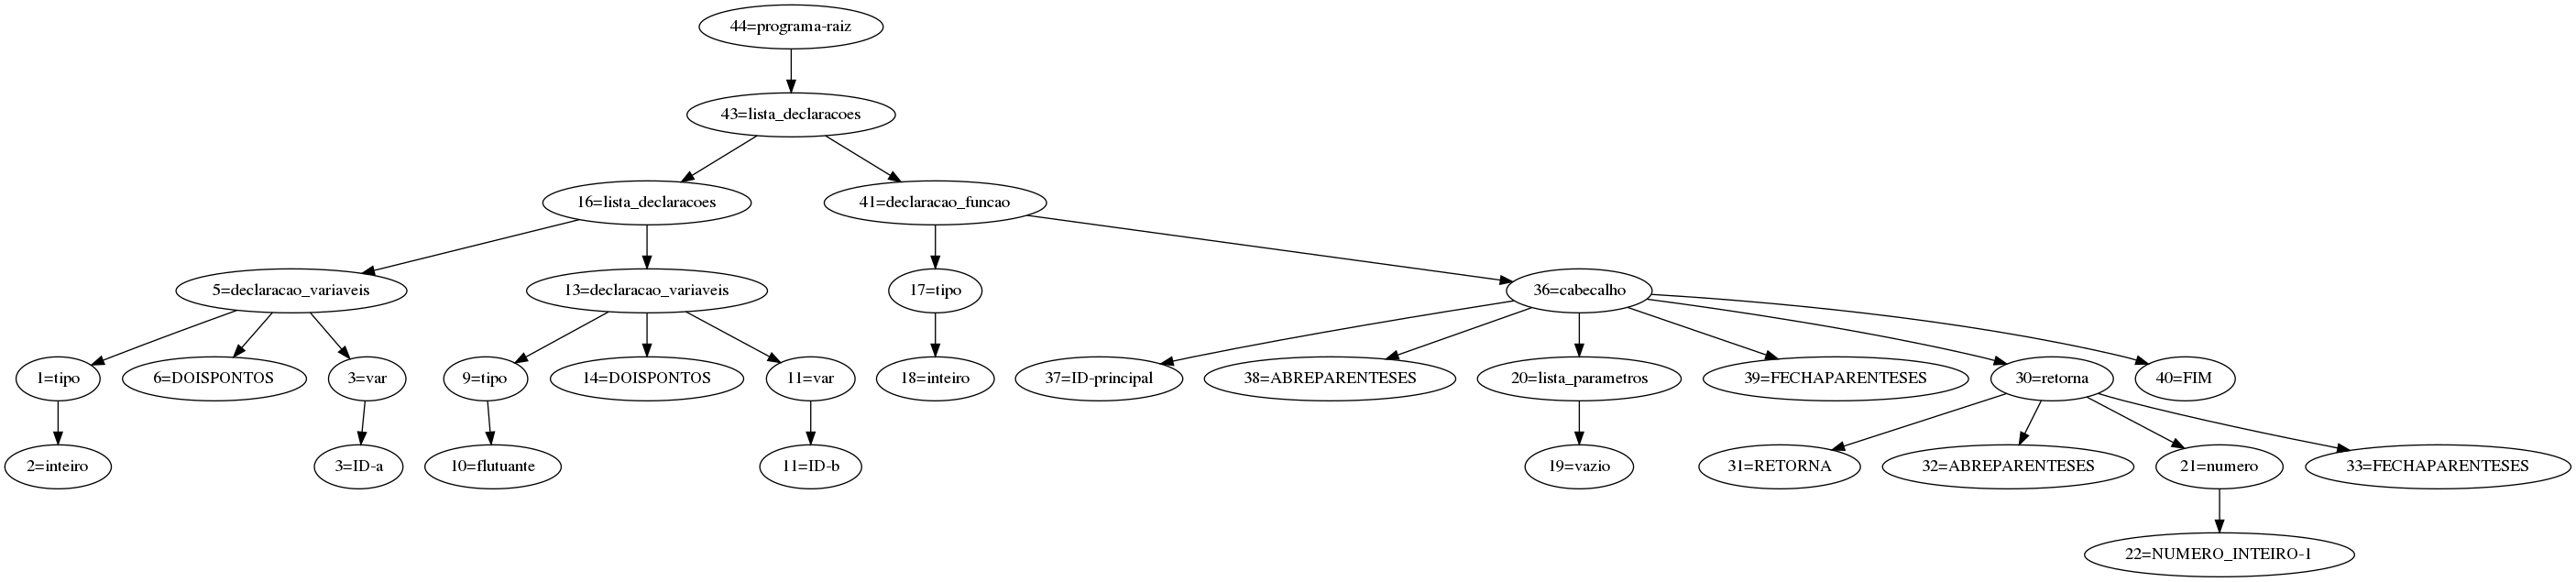
\includegraphics[width=\textwidth]{arvore-sintatica2} 
	\label{fig:arvoresimplificada}
\end{figure}
%  

\section{Geração de Código} 
A última etapa do processo de compilação da linguagem T++ trata-se da geração de código executável à partir do código binário. Neste caso usaremos a árvore sintática (após o processamento semântico) para gerar o código binário e então o executável do programa. 

O arquivo ``gencode.py'' contém as informações sobre a biblioteca para geração de código no Python:   
\begin{lstlisting}[language= Python, caption= Bibliotecas para geração de código em Python, label=cod:coddp] 
from llvmlite import ir   
from llvmlite import binding as llvm    

def codegen():
	llvm.initialize()
	llvm.initialize_all_targets()
	llvm.initialize_native_target()
	llvm.initialize_native_asmprinter()  
	module = ir.Module('geracao-codigo-tpp.bc')  
	module.triple = llvm.get_default_triple()
	
	target = llvm.Target.from_triple(module.triple)
	target_machine = target.create_target_machine() 
	module.data_layout = target_machine.target_data   
	
	t_int = ir.IntType(32) 
	t_func = ir.FunctionType(t_int, ()) 
	# Cria o módulo.
	module = ir.Module('meu_modulo.bc')
	arquivo = open('meu_modulo.ll', 'w')
	arquivo.write(str(module))
	arquivo.close()
	print(module) 
\end{lstlisting} 


\subsection{Execução dos testes de geração de código}  
Para visualização do processo de geração de código será utilizado o seguinte programa na linguagem nova tpp: 

\begin{lstlisting}[language=bash, caption=Programa na linguagem tpp] 

inteiro soma(inteiro: x, inteiro: y)
retorna(x + y)
fim

inteiro sub(inteiro: z, inteiro: t)
	retorna(z + t)
fim

inteiro principal()
	inteiro: a
	inteiro: b
	inteiro: c
	inteiro: i
	
	i := 0
	
	repita
	leia(a)
	leia(b)
	c := soma(soma(a,b), sub(a,b))
	escreva(c)
	i := i + 1
	até i = 5
	
	retorna(0)
fim
\end{lstlisting}

Após percorrer o todos os processos (léxico, sintático, semântico e geração de código) então o executável do programa é gerado.
Os testes podem ser executados como o seguinte comando: 
\begin{lstlisting}[language=bash, caption=Execução do códgio tpp no terminal]
$ python3 main.py geracao-codigo-testes/gencode-007.tpp 
$ sudo ./run.sh
\end{lstlisting}
O primeiro comando no terminal gera o código binário e então o segundo gera o executável.  

O seguinte arquivo será gerado em ``root.ll'':  

\begin{verbatim}
; ModuleID = "geracao-codigo-tpp.bc"
target triple = "x86_64-unknown-linux-gnu"
target datalayout = ""

define i32 @"soma"(i32 %"x", i32 %"y") 
{
entry:
	%"x.1" = alloca i32
	%"y.1" = alloca i32
	%".4" = load i32, i32* %"x.1"
	%".5" = load i32, i32* %"y.1"
	%"add" = add i32 %".4", %".5"
	br label %"exit"
exit:
	%".7" = add i32 %"x", %"y"
	ret i32 %".7"
}

define i32 @"sub"(i32 %"z", i32 %"t") 
{
entry:
	%"z.1" = alloca i32
	%"t.1" = alloca i32
	%".4" = load i32, i32* %"z.1"
	%".5" = load i32, i32* %"t.1"
	%"add" = sub i32 %".4", %".5"
	br label %"exit"
exit:
	%".7" = add i32 %"z", %"t"
	ret i32 %".7"
}

define i32 @"main"() 
{
entry:
	%"a" = alloca i32, align 4
	%"b" = alloca i32, align 4
	%"c" = alloca i32, align 4
	%"i" = alloca i32, align 4
	store i32 0, i32* %"i"
	br label %"repita_inicio"
	repita_inicio:
	%".4" = load i32, i32* %"i"
	%"1" = alloca i32
	%".5" = load i32, i32* %"1"
	%"incremento" = add i32 %".4", %".5"
	%".6" = load i32, i32* %"i"
	%"result" = add i32 %".6", 1
	store i32 %"result", i32* %"i"
	%".8" = load i32, i32* %"a"
	%".9" = load i32, i32* %"b"
	%".10" = call i32 @"soma"(i32 %".8", i32 %".9")
	%".11" = load i32, i32* %"a"
	%".12" = load i32, i32* %"b"
	%".13" = call i32 @"sub"(i32 %".11", i32 %".12")
	%".14" = call i32 @"soma"(i32 %".10", i32 %".13")
	%"b_cmp" = load i32, i32* %"i", align 4
	%"if_test_while" = icmp eq i32 %"b_cmp", 5
	br i1 %"if_test_while", label %"repita_fim", label %"repita_inicio"
repita_fim:
	br label %"exit"
exit:
ret i32 0
}

declare void @"escreva_valor(c)"() 

declare i32 @"leiaInteiro (a)"(i8* %".1", ...) 

declare i32 @"leiaInteiro (b)"(i8* %".1", ...) 

\end{verbatim}

\bibliographystyle{sbc}

\begin{thebibliography}{99} 
	\bibitem[louden]{louden} 
	LOUDEN, Kenneth C. 2004. \textit{Compiladores}: Princípios e Práticas. 1st ed.
	São Paulo, SP: Thomson. 
	\bibitem[]{buerger1989latex}  
	\textbf{Syntax Highlight Guide}. Acesso em 2019. Disponível em: \url{
		https://code.visualstudio.com/api/language-extensions/syntax-highlight-guide} 
	\bibitem[JARGAS]{automatos}[JARGAS] JARGAS, Aurélio Marinho. 2012. Expressões regulares: uma abordagem divertida. 4 ed. São
	Paulo, SP: Novatec.
	\bibitem[Yacc]{yacc}[Yacc]. Johnson, Stephen C. [1975]. Yacc: Yet Another Compiler
	Compiler. Computing Science Technical Report No. 32, Bell
	Laboratories, Murray hill, New Jersey. A PDF version is available at
	ePaperPress.  
	%BUERGER, D. J.LATEX for scientists and engineers. EUA: McGraw-Hill, 1989. 198 p.
	%\bibitem{miktex2009}   
	%SCHENK, C. et al. Mik\TeX. 2009. Programa de computador. Disponível em: \url{<https://miktex.org}. Acesso em:  07/03/2019.
	%\bibitem{knu84} Knuth, D. E., The TeXbook, Addison Wesley, 1984. 
\end{thebibliography}
\end{document}